\documentclass[aspectratio=169]{beamer}

\usepackage{fontspec}
\setmainfont{Latin Modern Roman}
\setsansfont{Latin Modern Sans}
\setmonofont{Latin Modern Mono}
\usepackage{polyglossia}
\setdefaultlanguage{vietnamese}
\usepackage{booktabs}
\usepackage{graphicx}
\usepackage{xcolor}
\usepackage{tikz}
\usetikzlibrary{arrows.meta,positioning}

\definecolor{primaryBlue}{HTML}{3636AE}
\definecolor{darkBlue}{HTML}{262686}
\definecolor{accentGreen}{HTML}{168C72}
\usetheme{Madrid}
\usecolortheme[named=primaryBlue]{structure}
\setbeamertemplate{navigation symbols}{}
\setbeamercolor{alerted text}{fg=darkBlue}
\setbeamercolor{block title alerted}{bg=darkBlue,fg=white}
\setbeamercolor{block body alerted}{bg=primaryBlue!8,fg=black}
\setbeamercolor{block title example}{bg=accentGreen,fg=white}
\setbeamercolor{block body example}{bg=accentGreen!8,fg=black}

\title[Dự báo PM2.5 đa chân trời]{\textbf{Xây dựng và Triển khai Hệ thống Học máy Ứng dụng}}
\subtitle{Dự báo PM2.5 đa chân trời từ 1 đến 24 giờ tại Việt Nam}
\author[Nhóm 11]{Nhóm 11\\\small T.K. Ngọc, N.T. Nguyên, N.M. Thắng, T.Đ. Luân, N.T. Nhân}
\institute[KHTN TP.HCM]{Nhập môn Học máy - Đại học Khoa học Tự nhiên TP.HCM}
\date{Năm học 2025--2026}

\begin{document}

\begin{frame}\titlepage\end{frame}

\begin{frame}{Thông tin nhóm và phân công công việc}
\small
\begin{table}
\begin{tabular}{lcl}
\toprule
Họ và tên & MSSV & Nhiệm vụ chính\\
\midrule
Trần Kim Ngọc & 23120062 & Ý tưởng, crawl dữ liệu, báo cáo và slide\\
Nguyễn Thành Nguyên & 23120063 & Tiền xử lý, EDA, feature engineering\\
Nguyễn Mạnh Thắng & 23120084 & SARIMAX, temporal split, phân tích lỗi\\
Trần Đình Luân & 23120059 & LSTM đa đầu ra, learning curves\\
Nguyễn Thiện Nhân & 23120064 & XGBoost, FastAPI, React, Docker\\
\bottomrule
\end{tabular}
\end{table}
\end{frame}

\begin{frame}{Nội dung trình bày}\tableofcontents\end{frame}

\section{1. Bài toán và mục tiêu}
\begin{frame}{1. Bài toán và mục tiêu}{Từ một mốc $t+24$ sang đường dự báo 24 giờ}
\begin{columns}[T]
\begin{column}{0.57\textwidth}
\begin{itemize}
\item \textbf{Bản cũ:} chỉ dự báo PM2.5 tại $t+24$.
\item \textbf{Bản mới:} dự báo đồng thời $t+1,t+2,\ldots,t+24$.
\item \textbf{Target:} PM2.5 liên tục, không phải PM2.5 hiện tại và không phải AQI.
\item \textbf{Giá trị thực tiễn:} người dùng chọn đúng giờ cần đi lại hoặc hoạt động ngoài trời.
\end{itemize}
\end{column}
\begin{column}{0.41\textwidth}
\begin{alertblock}{Đầu ra tại origin $t$}
\[
\hat{\mathbf y}_t=[\hat y_{t+1},\ldots,\hat y_{t+24}]
\]
24 giá trị PM2.5, đơn vị $\mu$g/m$^3$.
\end{alertblock}
\end{column}
\end{columns}
\end{frame}

\begin{frame}{1. Bài toán và mục tiêu}{Vì sao dự báo trực tiếp PM2.5?}
\begin{columns}[T]
\begin{column}{0.48\textwidth}
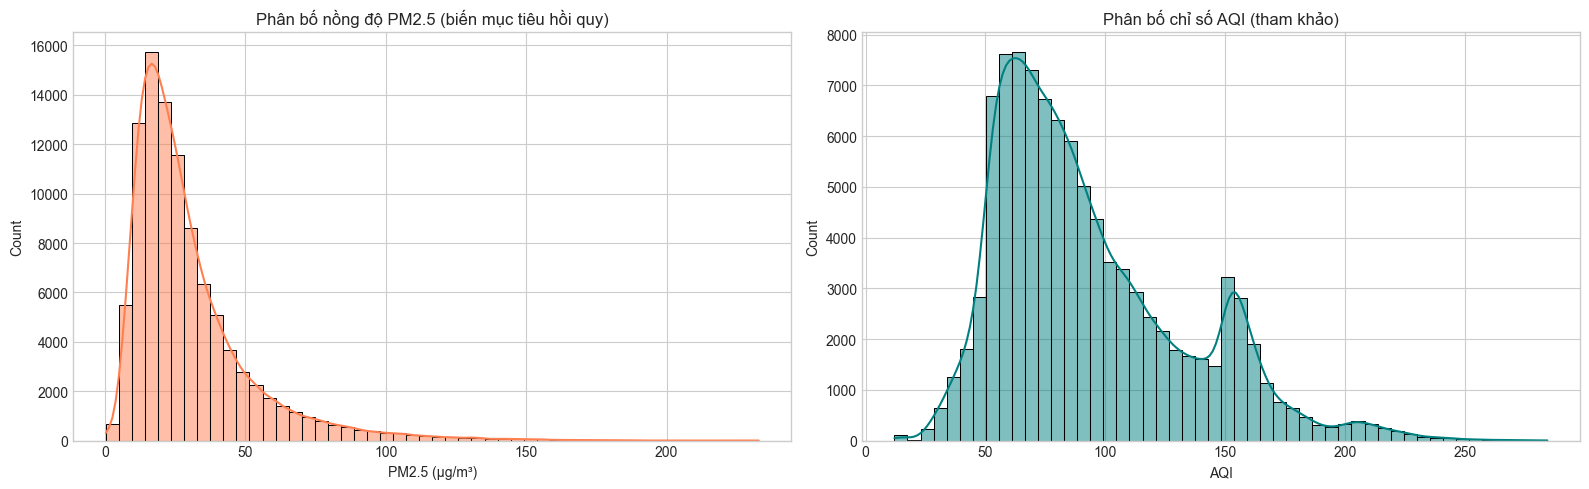
\includegraphics[width=\linewidth]{figures/eda_pm25_aqi_distributions.png}
\centering\scriptsize Phân phối PM2.5 và AQI
\end{column}
\begin{column}{0.48\textwidth}
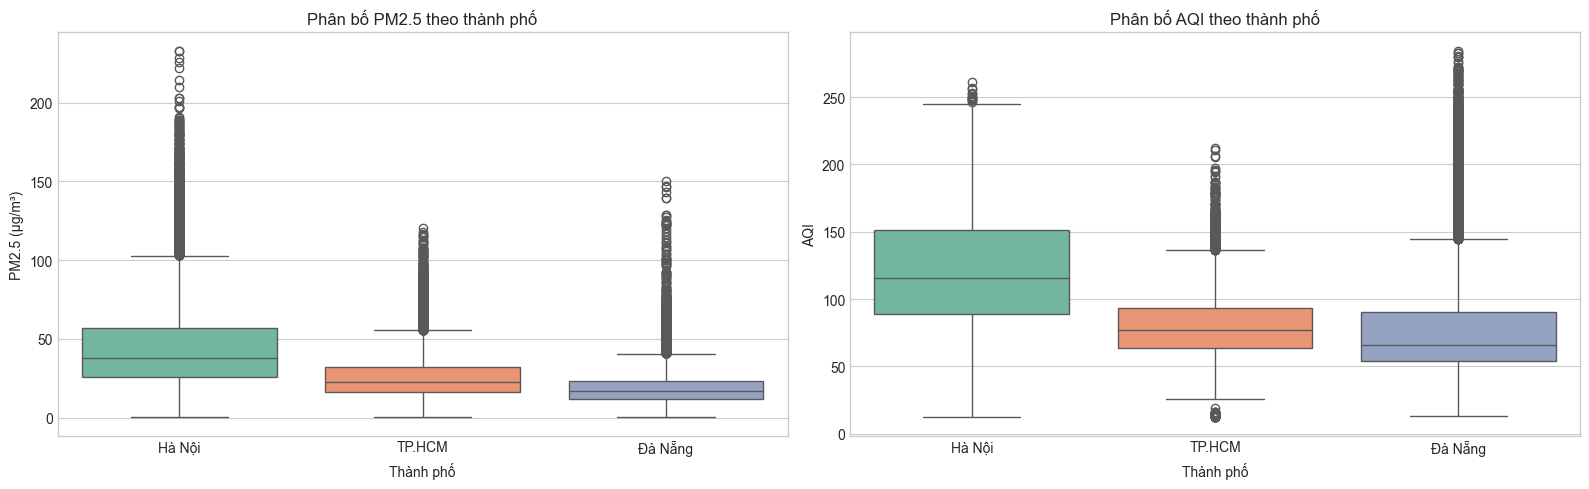
\includegraphics[width=\linewidth]{figures/eda_pm25_aqi_boxplots.png}
\centering\scriptsize Độ phân tán và cực trị
\end{column}
\end{columns}
\begin{block}{Kết luận target}
PM2.5 giữ biên độ vật lý và các đỉnh bụi mịn cần cảnh báo; AQI chỉ dùng tham chiếu trong EDA.
\end{block}
\end{frame}

\begin{frame}{1. Bài toán và mục tiêu}{Cấu trúc thời gian của PM2.5}
\begin{columns}[T]
\begin{column}{0.32\textwidth}\centering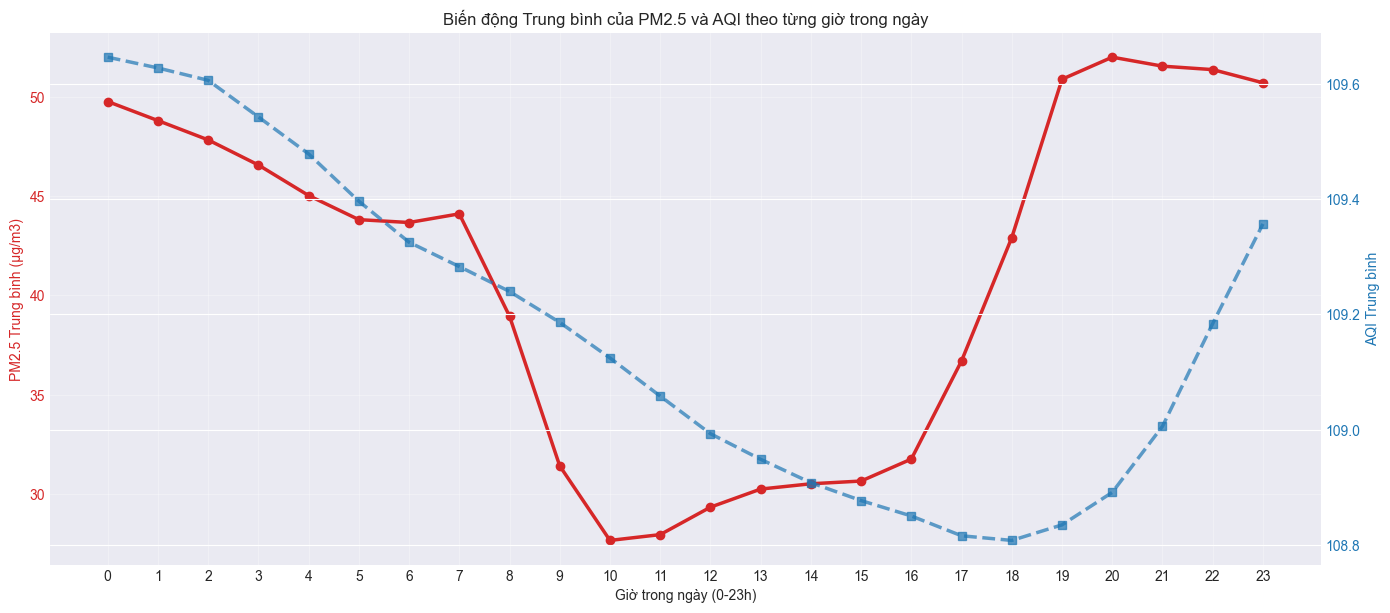
\includegraphics[width=\linewidth,height=0.42\textheight,keepaspectratio]{figures/pm25_aqi_hourly_profile.png}\par\scriptsize Hồ sơ theo giờ\end{column}
\begin{column}{0.32\textwidth}\centering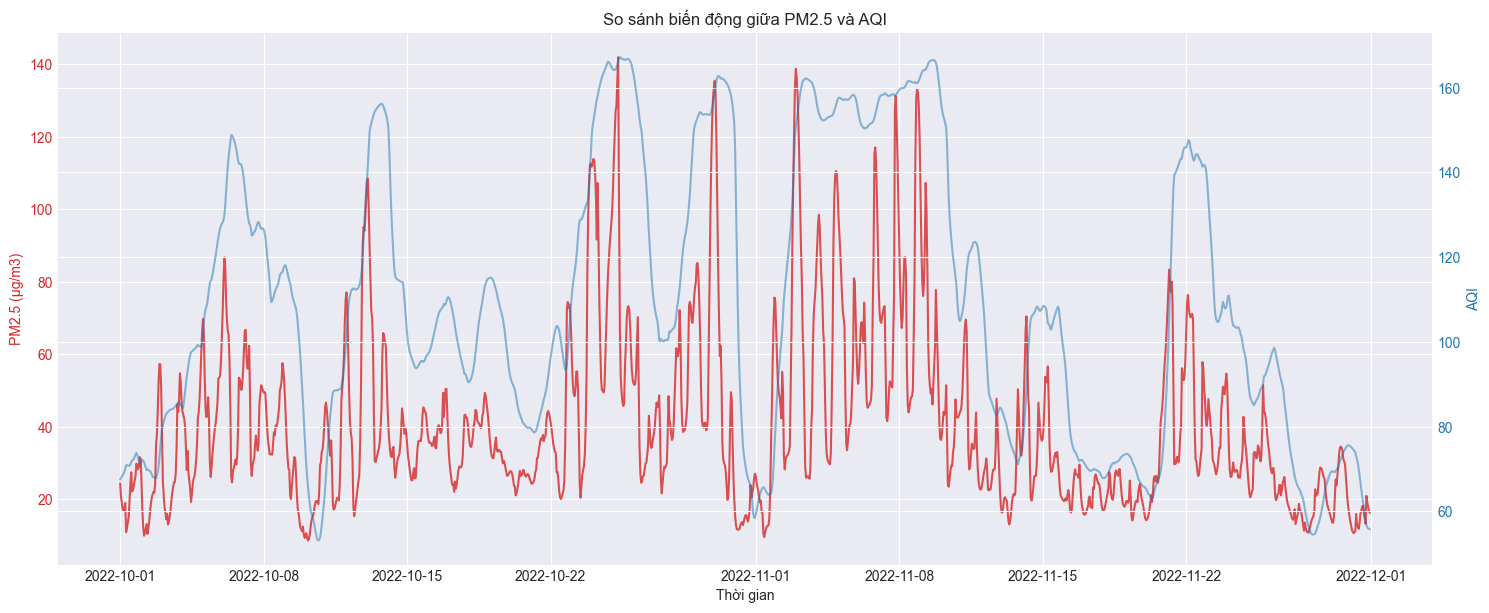
\includegraphics[width=\linewidth,height=0.42\textheight,keepaspectratio]{figures/pm25_aqi_timeseries.png}\par\scriptsize Chuỗi thời gian\end{column}
\begin{column}{0.32\textwidth}\centering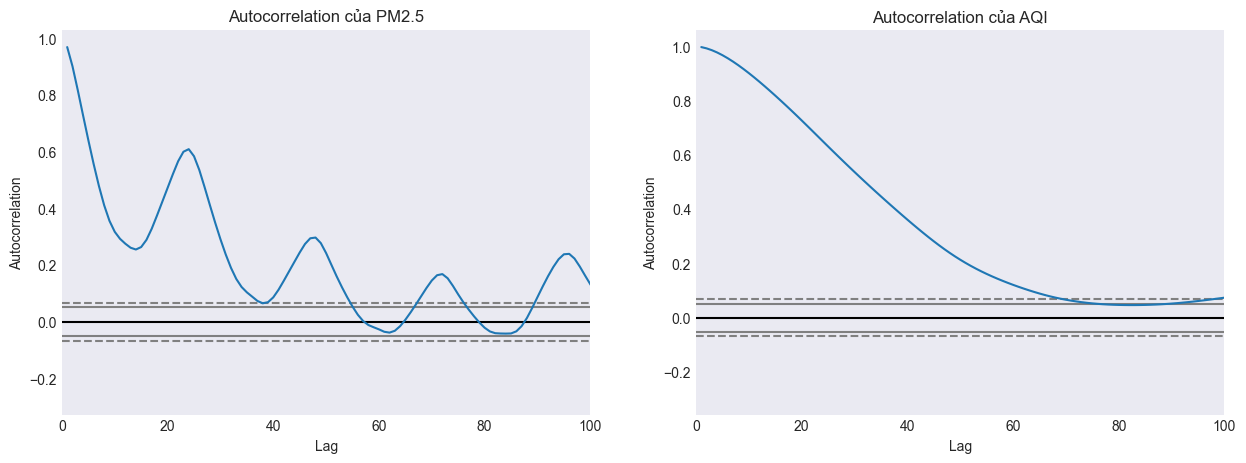
\includegraphics[width=\linewidth,height=0.42\textheight,keepaspectratio]{figures/pm25_aqi_autocorrelation.png}\par\scriptsize Tự tương quan\end{column}
\end{columns}
\vspace{0.25cm}
\begin{itemize}
\item Tín hiệu có quán tính ngắn hạn, chu kỳ ngày và tuần.
\item Đây là cơ sở cho lag, rolling, seasonal SARIMAX và chuỗi đầu vào LSTM.
\end{itemize}
\end{frame}

\section{2. Dữ liệu và Feature Engineering}
\begin{frame}{2. Dữ liệu và Feature Engineering}{Nguồn và phạm vi dữ liệu}
\begin{itemize}
\item \textbf{Không khí:} Open-Meteo Air Quality API, CAMS Global cho PM2.5, PM10, O$_3$, NO$_2$, SO$_2$, CO.
\item \textbf{Khí tượng:} Open-Meteo Historical Weather API cho nhiệt độ, độ ẩm, gió, mưa, áp suất và mây.
\item \textbf{Phạm vi:} Hà Nội, TP.HCM, Đà Nẵng; dữ liệu theo giờ từ 05/08/2022 đến 09/05/2026.
\item \textbf{Quy mô:} 98.907 dòng; không có city--datetime trùng hoặc khoảng thời gian phi giờ.
\end{itemize}
\begin{alertblock}{Giới hạn đại diện}
CAMS là dữ liệu lưới khí quyển tại một điểm đại diện mỗi thành phố, không thay thế trạm mặt đất và không diễn giải ở cấp quận.
\end{alertblock}
\end{frame}

\begin{frame}{2. Dữ liệu và Feature Engineering}{EDA: Phân phối các biến đầu vào}
\centering
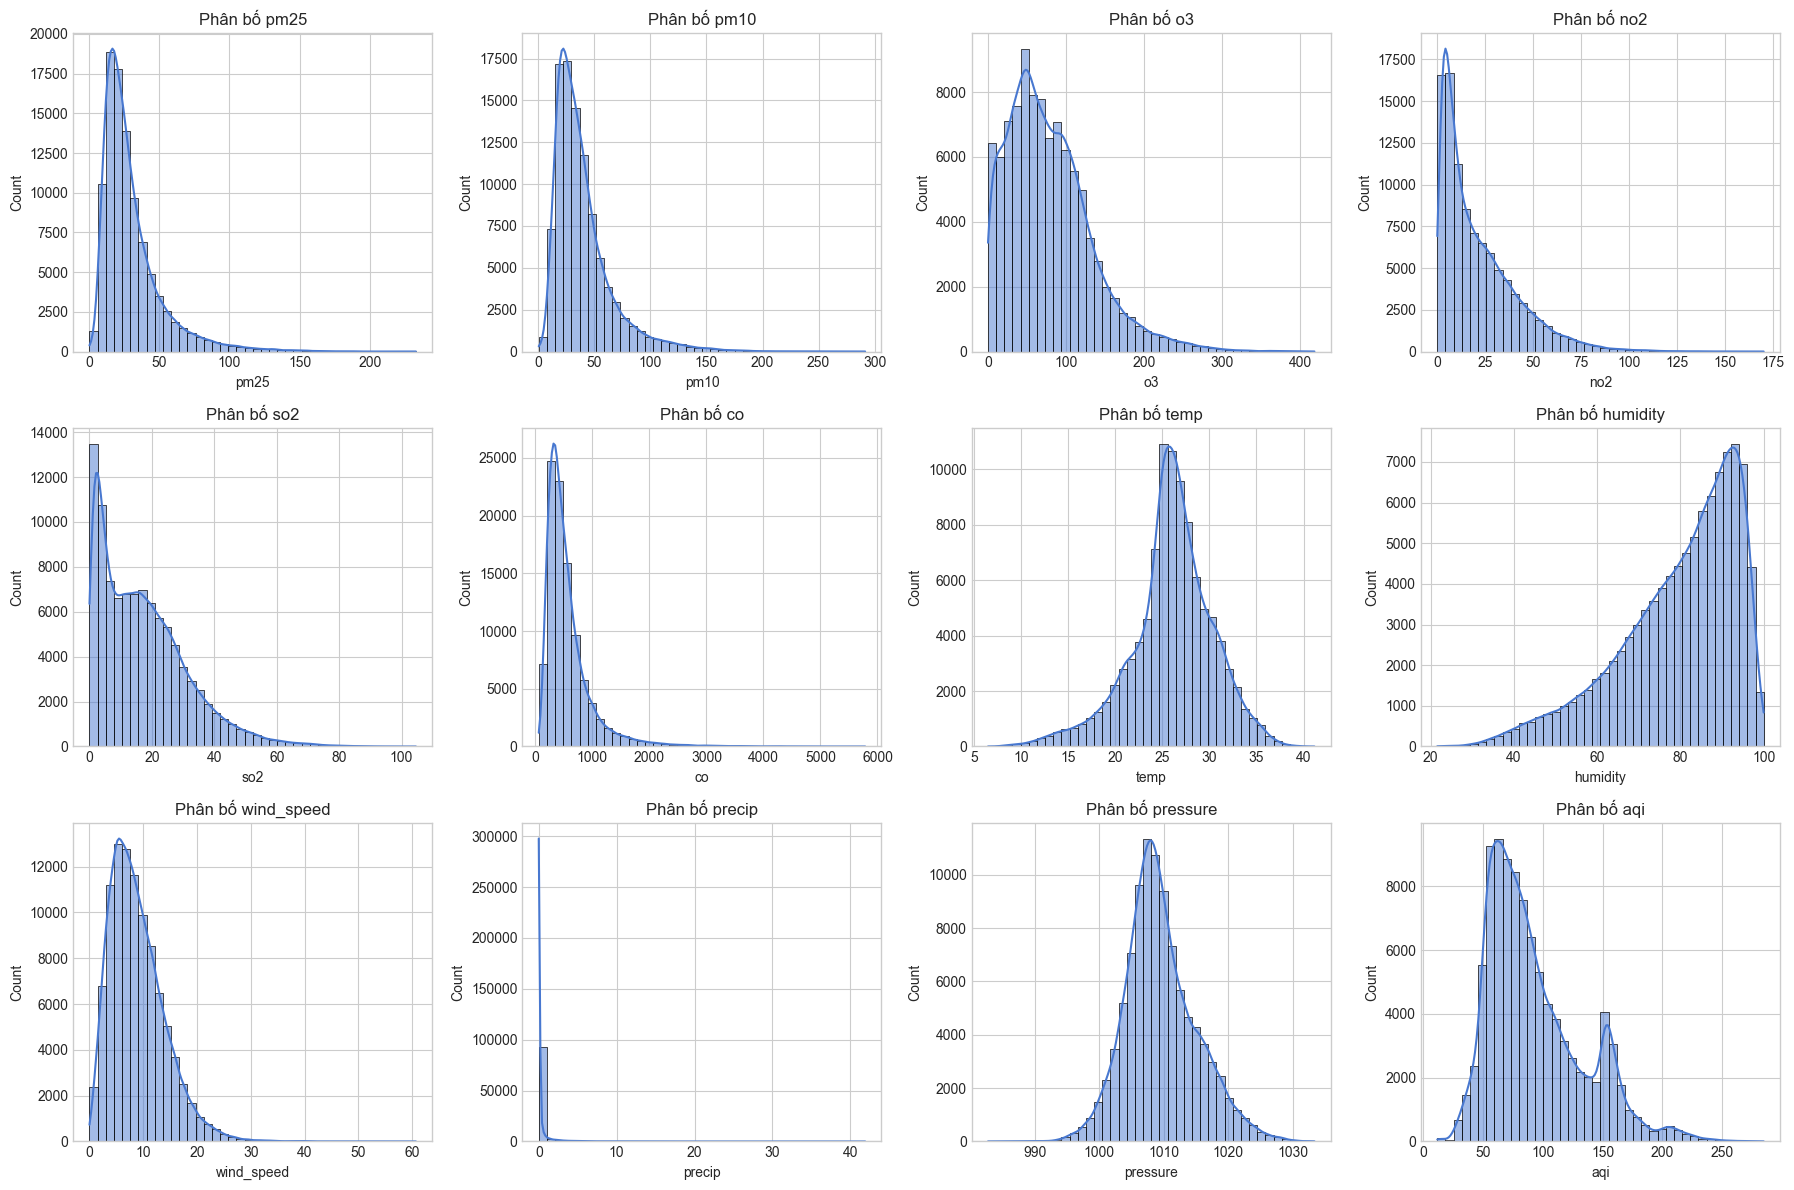
\includegraphics[width=0.88\linewidth,height=0.68\textheight,keepaspectratio]{figures/eda_feature_distributions.png}
\par\small Phân phối lệch và khác thang đo cho thấy cần kiểm tra ngoại lệ, đồng thời chuẩn hóa riêng cho LSTM.
\end{frame}

\begin{frame}{2. Dữ liệu và Feature Engineering}{EDA: Ma trận tương quan}
\centering
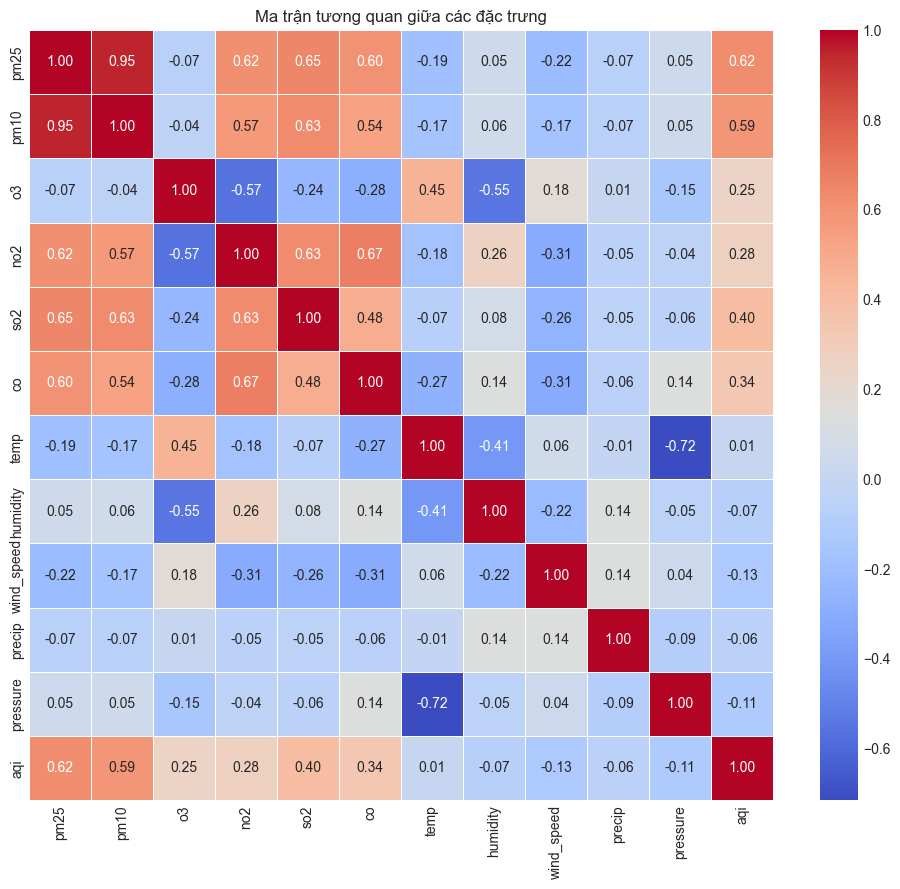
\includegraphics[width=0.66\linewidth,height=0.68\textheight,keepaspectratio]{figures/eda_correlation_heatmap.png}
\par\small PM2.5 tương quan cao với PM10; quan hệ khí tượng yếu hơn và có thể phi tuyến.
\end{frame}

\begin{frame}{2. Dữ liệu và Feature Engineering}{EDA: Ngoại lệ PM2.5}
\centering
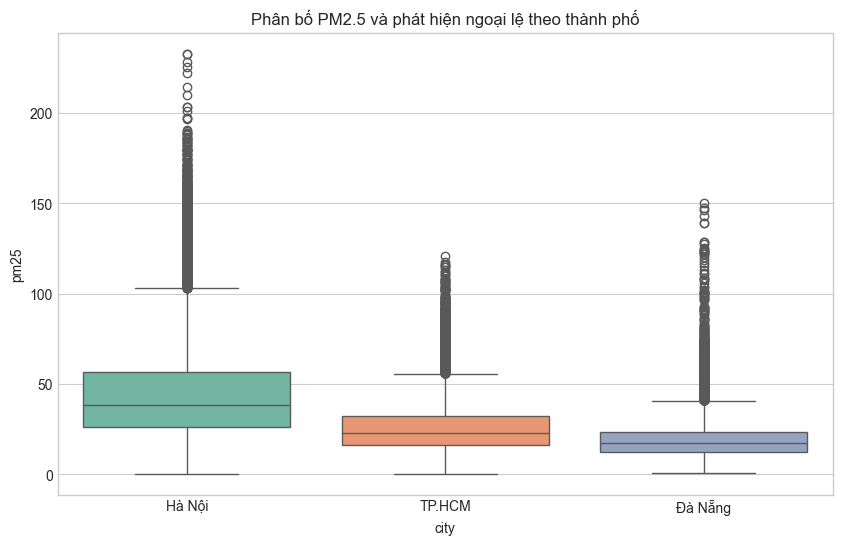
\includegraphics[width=0.88\linewidth,height=0.66\textheight,keepaspectratio]{figures/eda_pm25_outliers.png}
\par\small Các đỉnh hiếm được giữ lại vì đây là các tình huống ô nhiễm cần cảnh báo, không phải lỗi để cắt bỏ tự động.
\end{frame}

\begin{frame}{2. Dữ liệu và Feature Engineering}{EDA: Mẫu hình theo thời gian}
\centering
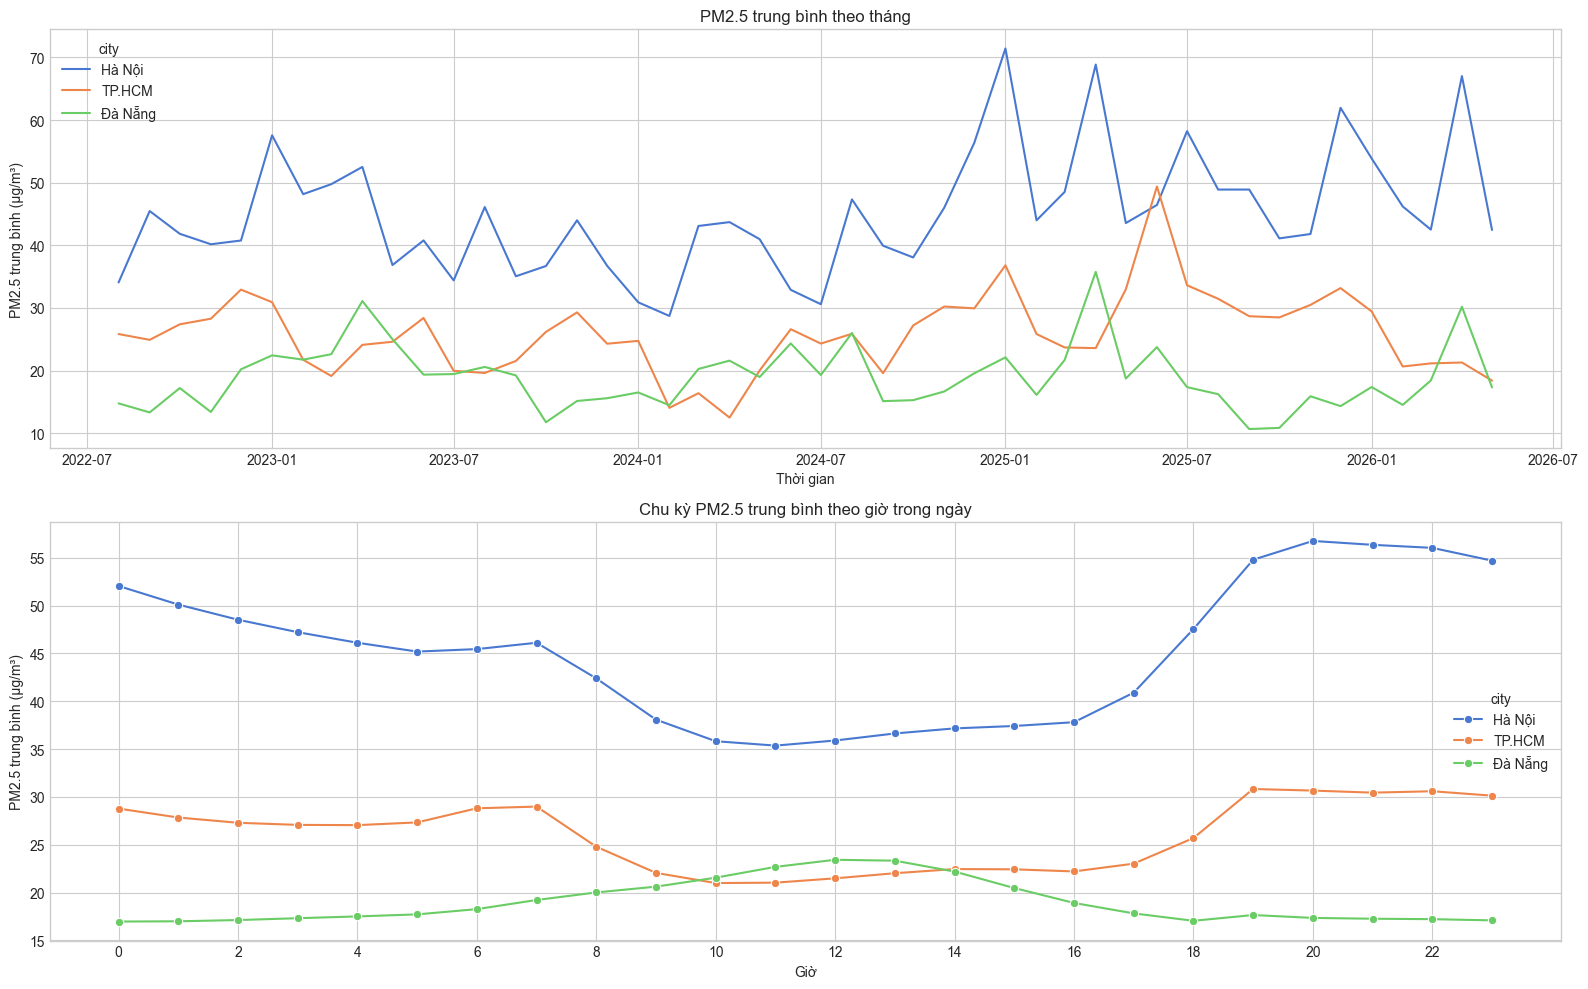
\includegraphics[width=0.90\linewidth,height=0.66\textheight,keepaspectratio]{figures/eda_pm25_temporal_patterns.png}
\par\small Chu kỳ theo giờ và tháng tạo cơ sở cho lag, rolling, biến sin/cos và seasonal SARIMAX.
\end{frame}

\begin{frame}{2. Dữ liệu và Feature Engineering}{Tiền xử lý và giải thích sáu class}
\small
\begin{columns}[T]
\begin{column}{0.51\textwidth}
\textbf{Tiền xử lý sau EDA}
\begin{itemize}
\item 13 giá trị O$_3$ âm $\rightarrow$ thiếu.
\item Nội suy tuyến tính riêng theo thành phố, tối đa 6 giờ.
\item Giữ các đỉnh PM2.5 hợp lệ.
\item Ghép target bằng đúng timestamp cùng thành phố.
\end{itemize}
\end{column}
\begin{column}{0.47\textwidth}
\textbf{Class do nhóm tự quy ước}
\begin{tabular}{lr}
Good & $\leq9.0$\\
Moderate & $9.0$--$35.4$\\
USG & $35.4$--$55.4$\\
Unhealthy & $55.4$--$125.4$\\
Very Unhealthy & $125.4$--$225.4$\\
Hazardous & $>225.4$\\
\end{tabular}
\end{column}
\end{columns}
\begin{alertblock}{Chỉ dùng để chẩn đoán}
Class được tạo sau dự đoán để lập confusion matrix; model vẫn hồi quy PM2.5 liên tục, không dự báo AQI.
\end{alertblock}
\end{frame}

\begin{frame}{2. Dữ liệu và Feature Engineering}{Feature Engineering đầy đủ}
\small
\begin{columns}[T]
\begin{column}{0.48\textwidth}
\textbf{Đặc trưng nguồn và lịch sử}
\begin{itemize}
\item 6 chất ô nhiễm, 7 biến khí tượng.
\item 5 biến thời gian.
\item 35 biến lịch sử PM2.5: lag 1--168 giờ; rolling 6--168 giờ; cùng giờ 7 ngày.
\end{itemize}
\end{column}
\begin{column}{0.48\textwidth}
\textbf{Đặc trưng phái sinh}
\begin{itemize}
\item Sin/cos giờ, ngày, tháng.
\item Delta và tỷ lệ rolling.
\item Ventilation, humid stagnation, mưa, gió yếu.
\item Wind vector, PM2.5/PM10, NO$_2$/CO.
\item One-hot thành phố và mùa.
\end{itemize}
\end{column}
\end{columns}
\begin{block}{Đầu ra}
75 cột sau mã hóa. Không feature nào sử dụng thông tin sau origin $t$.
\end{block}
\end{frame}

\begin{frame}{2. Dữ liệu và Feature Engineering}{Tạo target và chống rò rỉ}
\begin{columns}[T]
\begin{column}{0.50\textwidth}
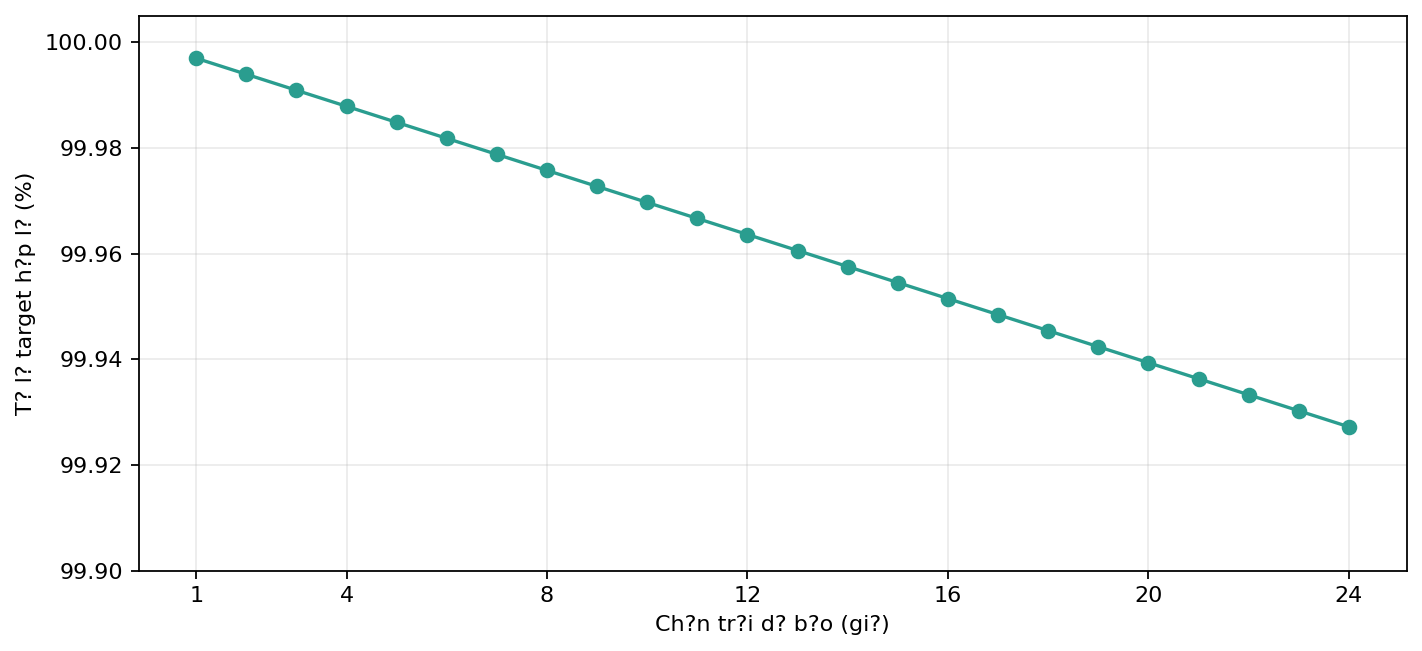
\includegraphics[width=\linewidth]{figures/target_coverage_by_horizon.png}
\centering\scriptsize Tỷ lệ target hợp lệ từ $t+1$ đến $t+24$
\end{column}
\begin{column}{0.47\textwidth}
\small
\begin{tabular}{lrr}
\toprule Tập & Origin & Tỷ lệ\\\midrule
Train & 68.829 & 70\%\\
Validation & 14.679 & 15\%\\
Test & 14.679 & 15\%\\\bottomrule
\end{tabular}
\vspace{0.25cm}
\begin{itemize}
\item Chia theo \texttt{forecast\_end}.
\item Purge gap 24 giờ giữa các tập.
\item Test bị khóa đến sau khi chọn model.
\end{itemize}
\end{column}
\end{columns}
\end{frame}

\section{3. Ba mô hình}
\begin{frame}{3. Ba mô hình}{SARIMAX đa bước}
\begin{itemize}
\item $\mathrm{SARIMAX}(1,0,0)\times(1,0,0)_{24}$, fit riêng cho từng thành phố.
\item Maximum likelihood, L-BFGS tối đa 200 vòng; cả ba thành phố hội tụ.
\item Dự báo đệ quy từ AR(1), seasonal AR(24) và lịch sử PM2.5.
\item \textbf{Ưu điểm:} baseline thời gian rõ ràng, tham số diễn giải được.
\item \textbf{Hạn chế:} giả định tuyến tính; lỗi đệ quy tích lũy ở horizon dài.
\end{itemize}
\end{frame}

\begin{frame}{3. Ba mô hình}{XGBoost Direct Multi-Horizon}
\small
\begin{itemize}
\item 24 XGBRegressor độc lập: model thứ $h$ học trực tiếp $PM2.5_{t+h}$.
\item 800 cây tối đa; learning rate 0,04; depth 3; min child weight 8.
\item Subsample và colsample 0,85; L1 0,05; L2 3,0.
\item Objective squared error, eval metric RMSE, early stopping 45 vòng.
\item \textbf{Ưu điểm:} học phi tuyến và tương tác; không truyền lỗi giữa horizon.
\item \textbf{Hạn chế:} 24 model riêng làm tăng thời gian huấn luyện và artifact.
\end{itemize}
\end{frame}

\begin{frame}{3. Ba mô hình}{LSTM Sequence-to-Vector}
\centering
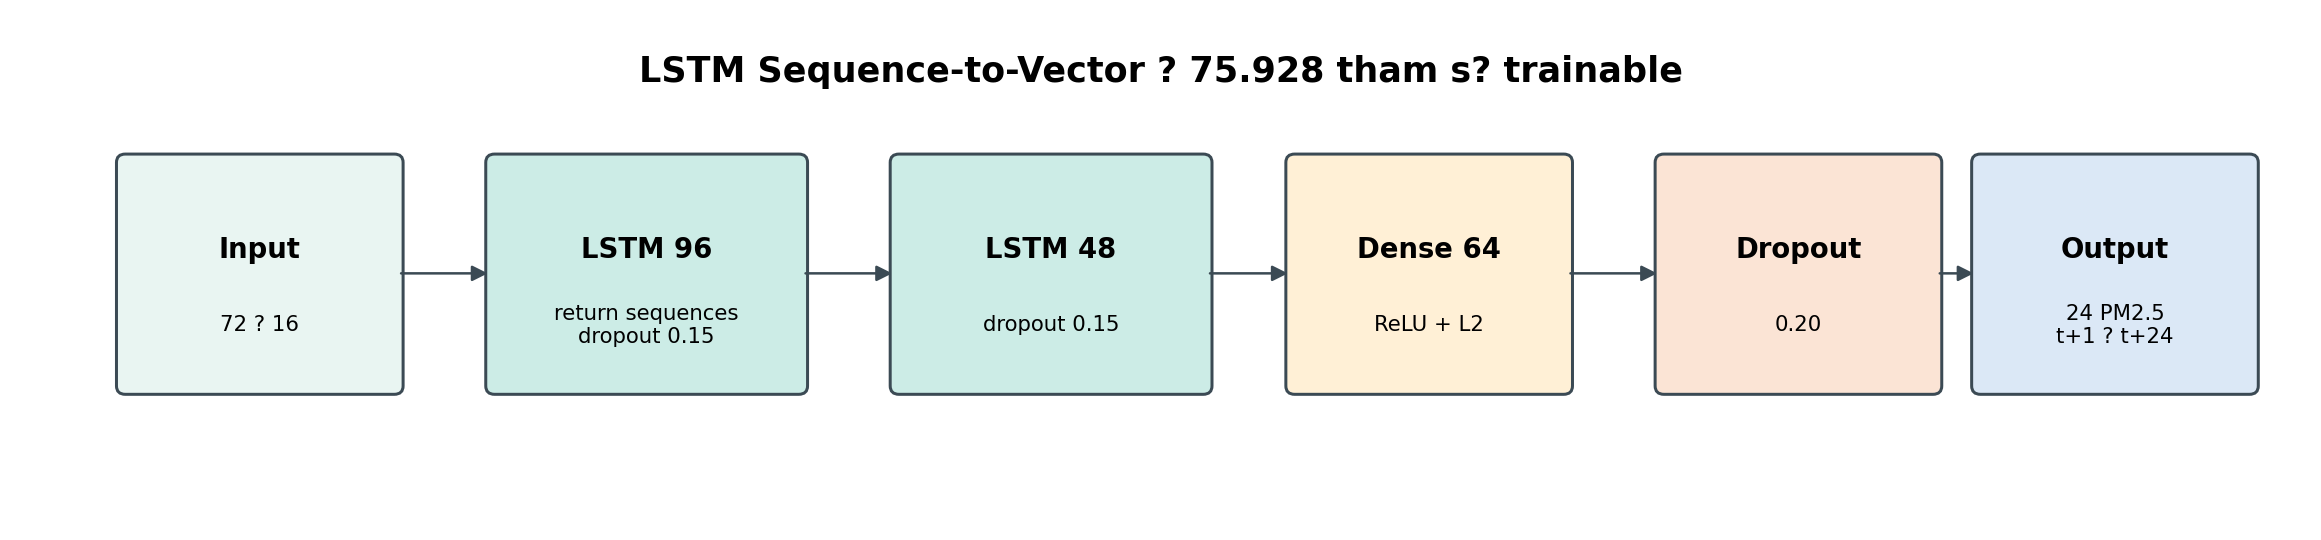
\includegraphics[width=0.96\linewidth]{figures/lstm_multihorizon_architecture.png}
\vspace{0.2cm}
\small Chuỗi 72 giờ $\times$ 16 feature $\rightarrow$ 24 đầu ra; 75.928 tham số trainable.
\end{frame}

\begin{frame}{3. Ba mô hình}{Cấu hình huấn luyện LSTM}
\begin{columns}[T]
\begin{column}{0.48\textwidth}
\begin{itemize}
\item Loss: MSE.
\item Metric: RMSE và MAE.
\item Adam, learning rate $10^{-3}$.
\item Batch 256, tối đa 60 epoch.
\end{itemize}
\end{column}
\begin{column}{0.48\textwidth}
\begin{itemize}
\item Early Stopping patience 10.
\item ReduceLROnPlateau patience 5.
\item L2 ở Dense và Dropout.
\item Không shuffle chuỗi thời gian.
\end{itemize}
\end{column}
\end{columns}
\begin{block}{Tuning}
Siêu tham số được chọn bằng Validation và regularization; Test không dùng để chỉnh cấu hình.
\end{block}
\end{frame}

\begin{frame}{3. Ba mô hình}{Learning curves LSTM}
\centering
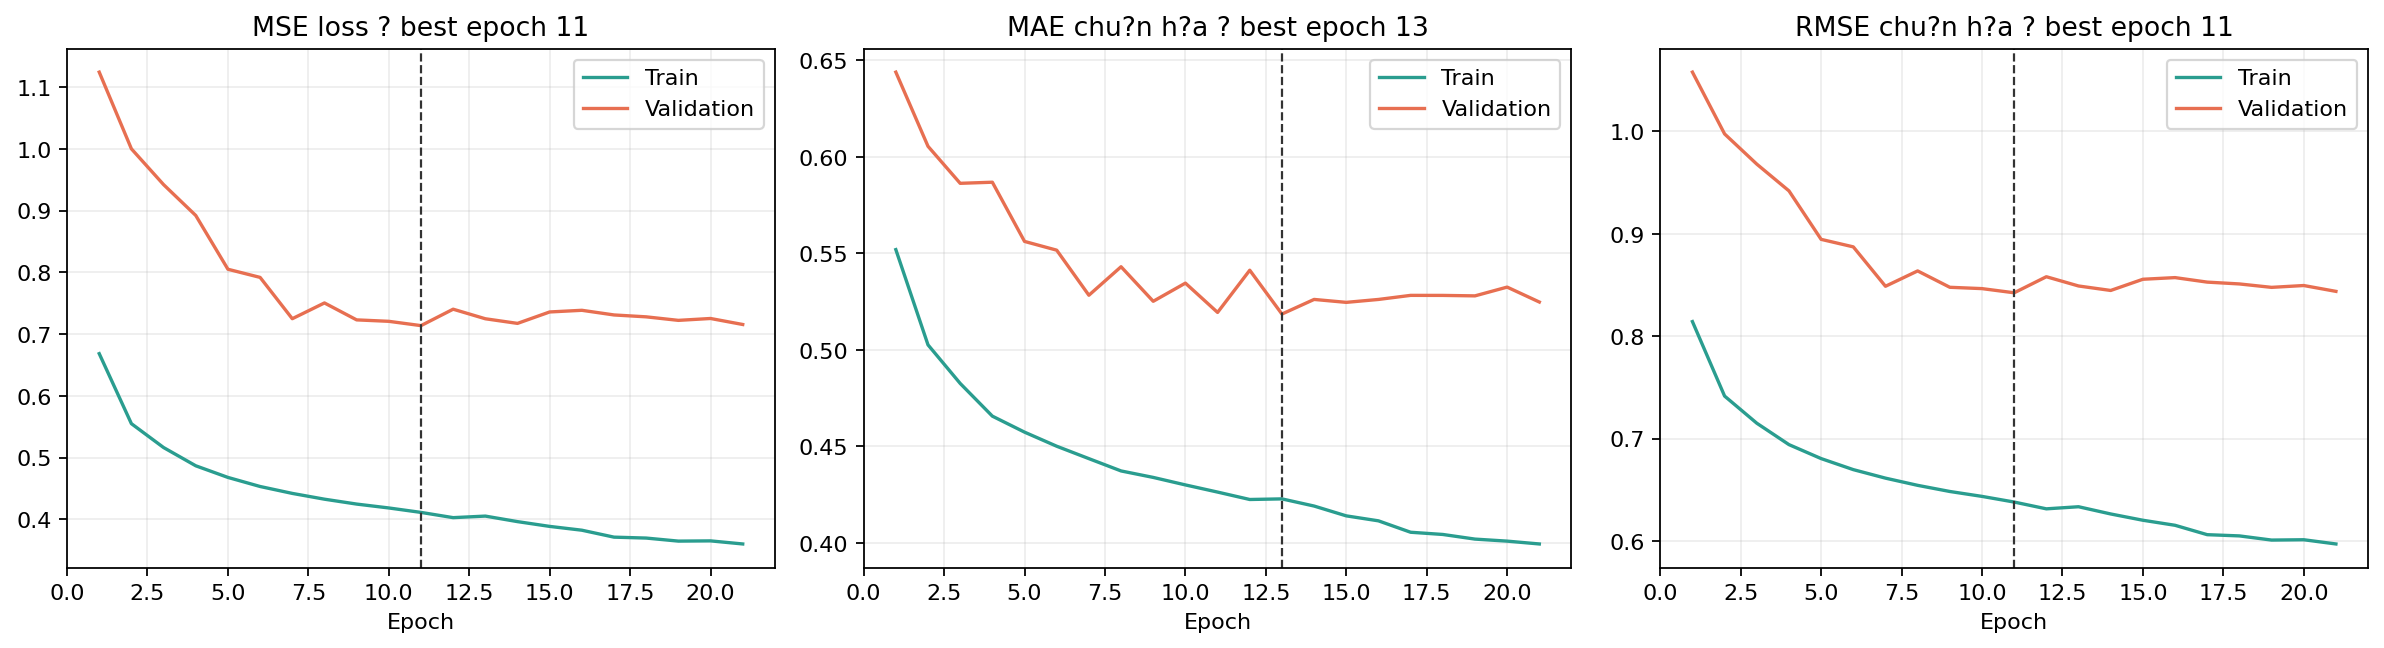
\includegraphics[width=0.98\linewidth]{figures/lstm_multihorizon_training_curves.png}
\small Validation loss tốt nhất tại epoch 11; Early Stopping khôi phục trọng số tốt nhất khi Train tiếp tục giảm.
\end{frame}

\section{4. Kết quả và thảo luận}
\begin{frame}{4. Kết quả và thảo luận}{Giao thức chọn model mới}
\begin{enumerate}
\item Chia Validation thành 5 khối thời gian liên tiếp, mỗi khối giữ đủ ba thành phố và 24 horizon.
\item Tính RMSE theo từng horizon rồi lấy trung bình trong mỗi fold.
\item Chọn theo mean CV RMSE; std, worst fold và MAE là tiêu chí phụ.
\item Khóa tên model trước khi mở Test.
\end{enumerate}
\begin{alertblock}{Giới hạn phương pháp}
Đây là blocked temporal validation trên candidate đã fit, không phải K-fold ngẫu nhiên và không tuyên bố refit cả ba model năm lần.
\end{alertblock}
\end{frame}

\begin{frame}{4. Kết quả và thảo luận}{Độ ổn định qua năm khối Validation}
\centering
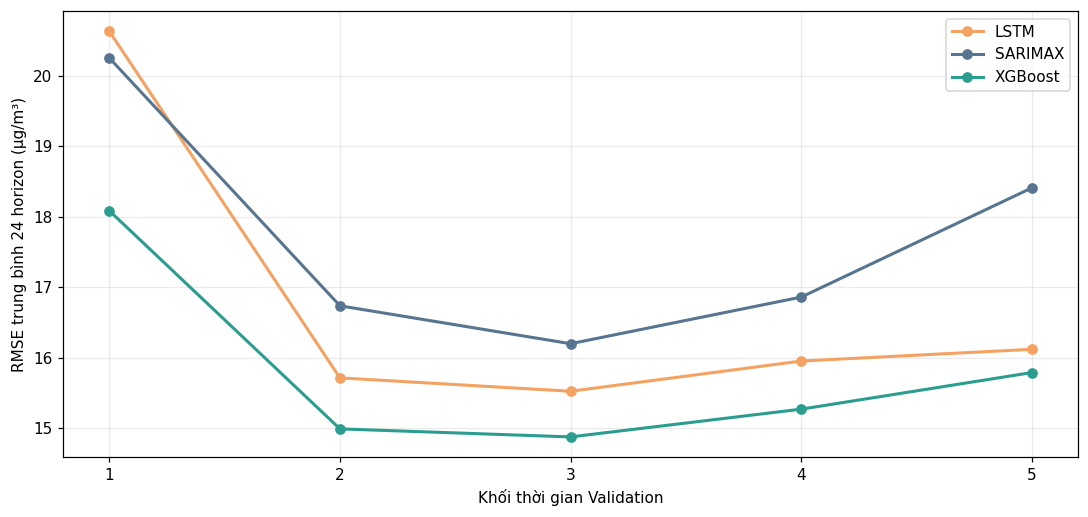
\includegraphics[width=0.88\linewidth]{figures/temporal_cv_fold_rmse.png}
\small XGBoost có RMSE thấp nhất ở cả 5/5 khối; kết luận không phụ thuộc một giai đoạn Validation đơn lẻ.
\end{frame}

\begin{frame}{4. Kết quả và thảo luận}{Kết quả lựa chọn model}
\begin{columns}[T]
\begin{column}{0.53\textwidth}
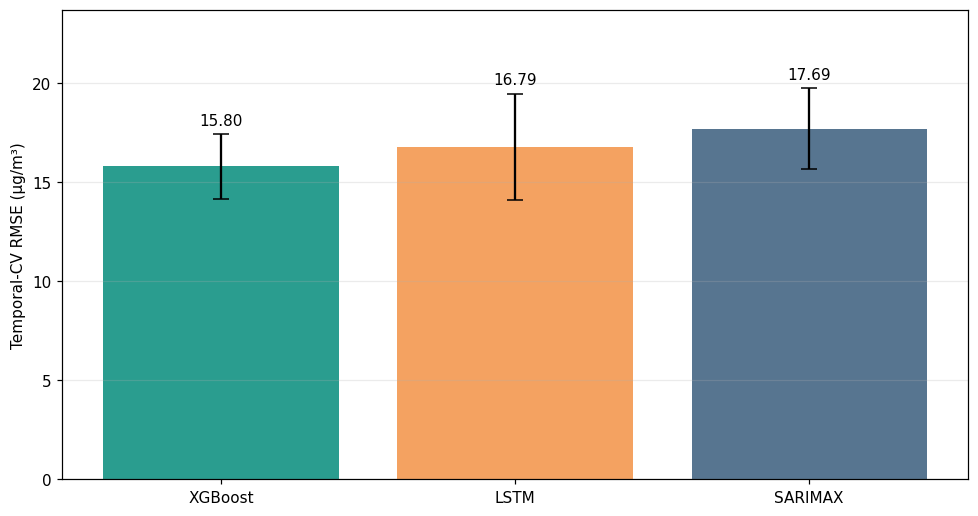
\includegraphics[width=\linewidth]{figures/temporal_cv_model_selection.png}
\end{column}
\begin{column}{0.44\textwidth}
\small
\begin{tabular}{lrr}
\toprule Model & CV RMSE & Std\\\midrule
\textbf{XGBoost} & \textbf{15,80} & 1,32\\
LSTM & 16,79 & 2,16\\
SARIMAX & 17,69 & 1,65\\\bottomrule
\end{tabular}
\vspace{0.25cm}
\begin{exampleblock}{Model được chọn}
XGBoost Direct Multi-Horizon.
\end{exampleblock}
\end{column}
\end{columns}
\end{frame}

\begin{frame}{4. Kết quả và thảo luận}{CV và Test sau khi khóa lựa chọn}
\begin{columns}[T]
\begin{column}{0.70\textwidth}
\centering
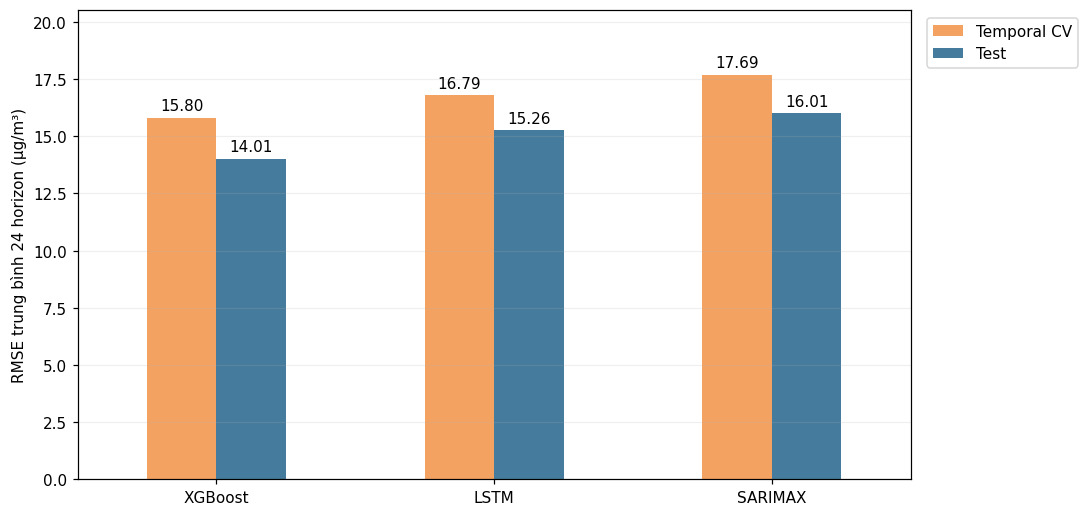
\includegraphics[width=\linewidth,height=0.68\textheight,keepaspectratio]{figures/cv_vs_test_model_comparison.png}
\end{column}
\begin{column}{0.27\textwidth}
\footnotesize
\begin{block}{Nguyên tắc}
Test chỉ được mở và báo cáo sau khi XGBoost thắng trên Validation.
\end{block}
\begin{exampleblock}{XGBoost trên Test}
RMSE: 14,01\\
MAE: 8,91\\
Global $R^2$: 0,665
\end{exampleblock}
\end{column}
\end{columns}
\end{frame}

\begin{frame}{4. Kết quả và thảo luận}{Sai số của ba model theo horizon}
\centering
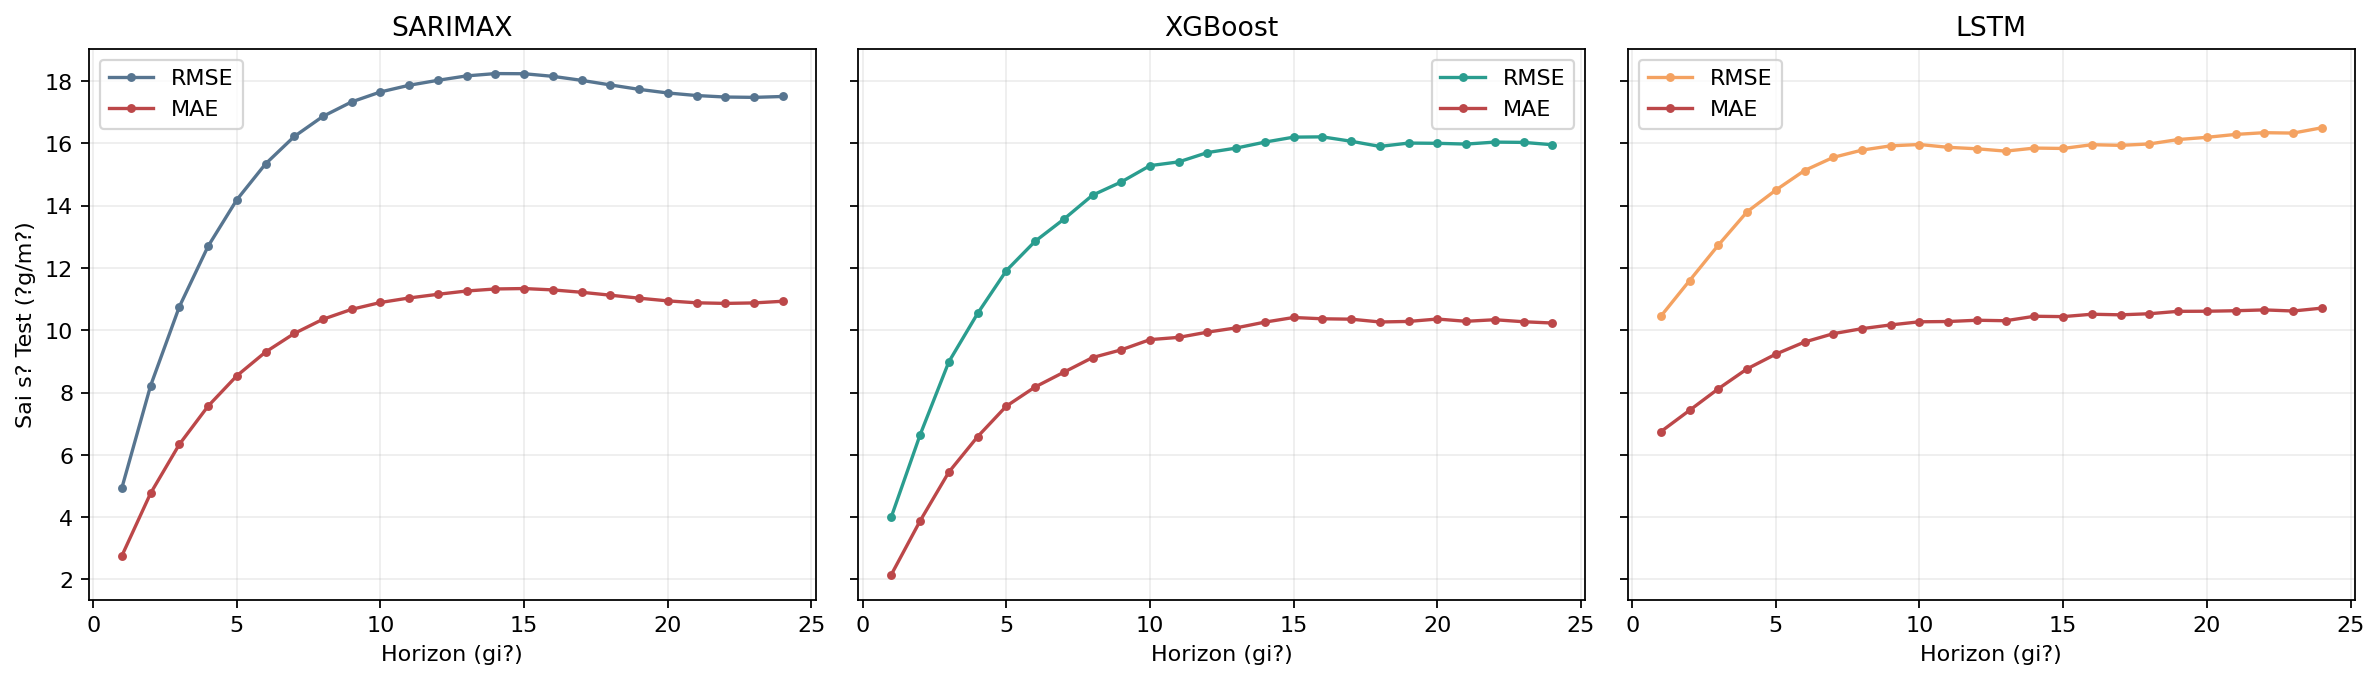
\includegraphics[width=0.98\linewidth]{figures/three_models_error_by_horizon.png}
\small Sai số tăng khi horizon dài; XGBoost có đường RMSE thấp nhất trên phần lớn dải 1--24 giờ.
\end{frame}

\begin{frame}{4. Kết quả và thảo luận}{XGBoost theo từng horizon}
\centering
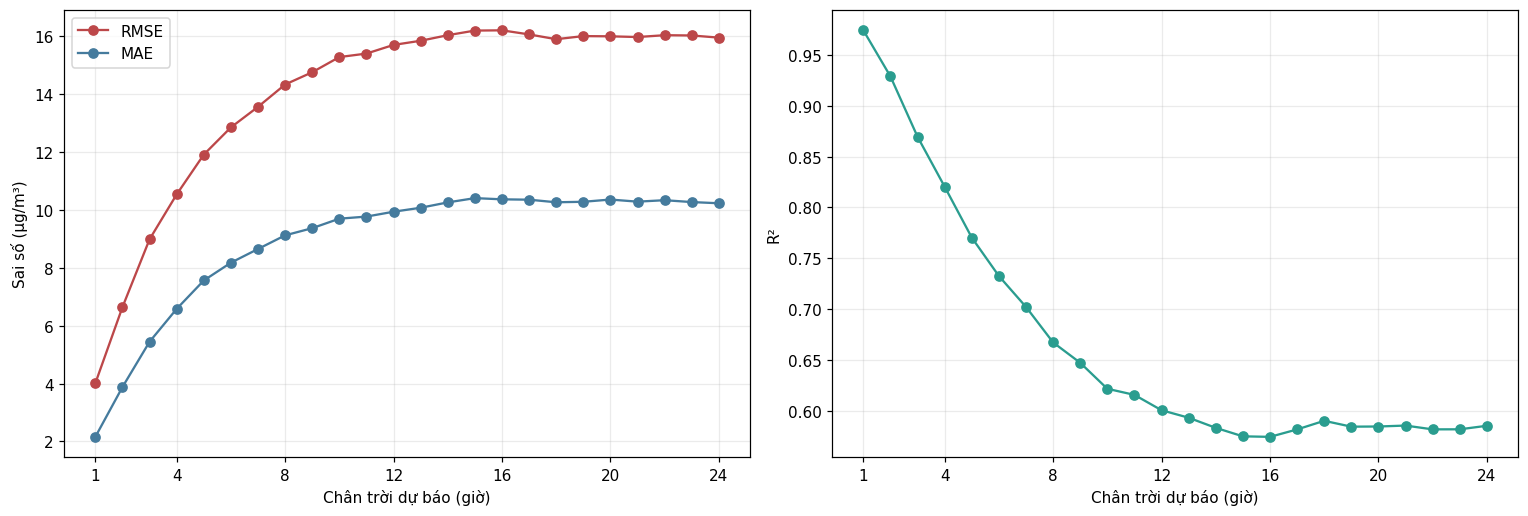
\includegraphics[width=0.92\linewidth]{figures/best_model_metrics_by_horizon.png}
\small RMSE tăng từ 4,01 ở $t+1$ lên 15,96 $\mu$g/m$^3$ ở $t+24$; khó nhất là $t+16$ với 16,21.
\end{frame}

\begin{frame}{4. Kết quả và thảo luận}{Độ ổn định theo thành phố}
\begin{columns}[T]
\begin{column}{0.58\textwidth}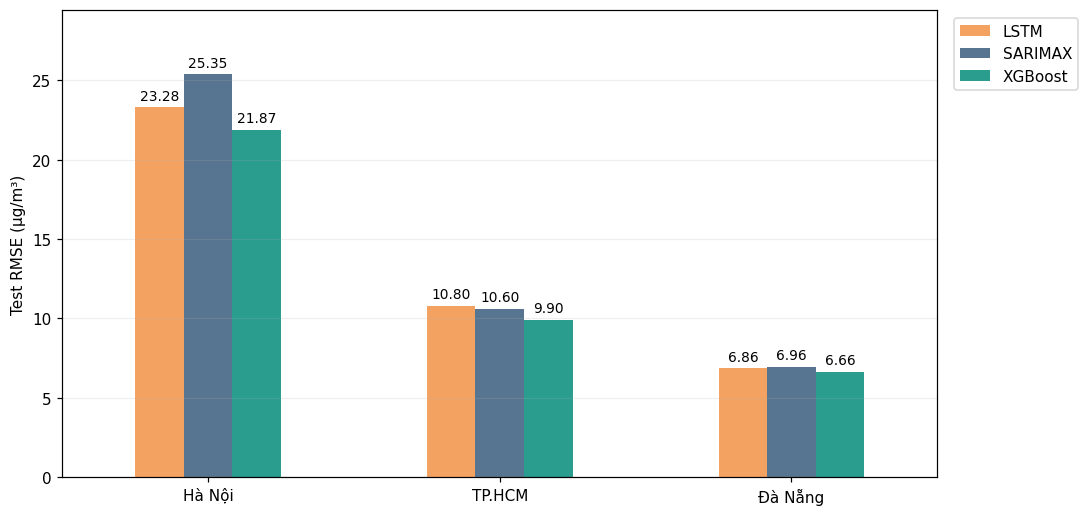
\includegraphics[width=\linewidth]{figures/test_rmse_by_city.png}\end{column}
\begin{column}{0.39\textwidth}
\begin{itemize}
\item Hà Nội: 21,87.
\item TP.HCM: 9,90.
\item Đà Nẵng: 6,66.
\end{itemize}
\begin{alertblock}{Failure mode}
Hà Nội có nhiều đỉnh và phương sai lớn; metric tổng hợp che giấu chênh lệch địa lý.
\end{alertblock}
\end{column}
\end{columns}
\end{frame}

\begin{frame}{4. Kết quả và thảo luận}{Learning curves XGBoost}
\begin{columns}[T]
\begin{column}{0.75\textwidth}
\centering
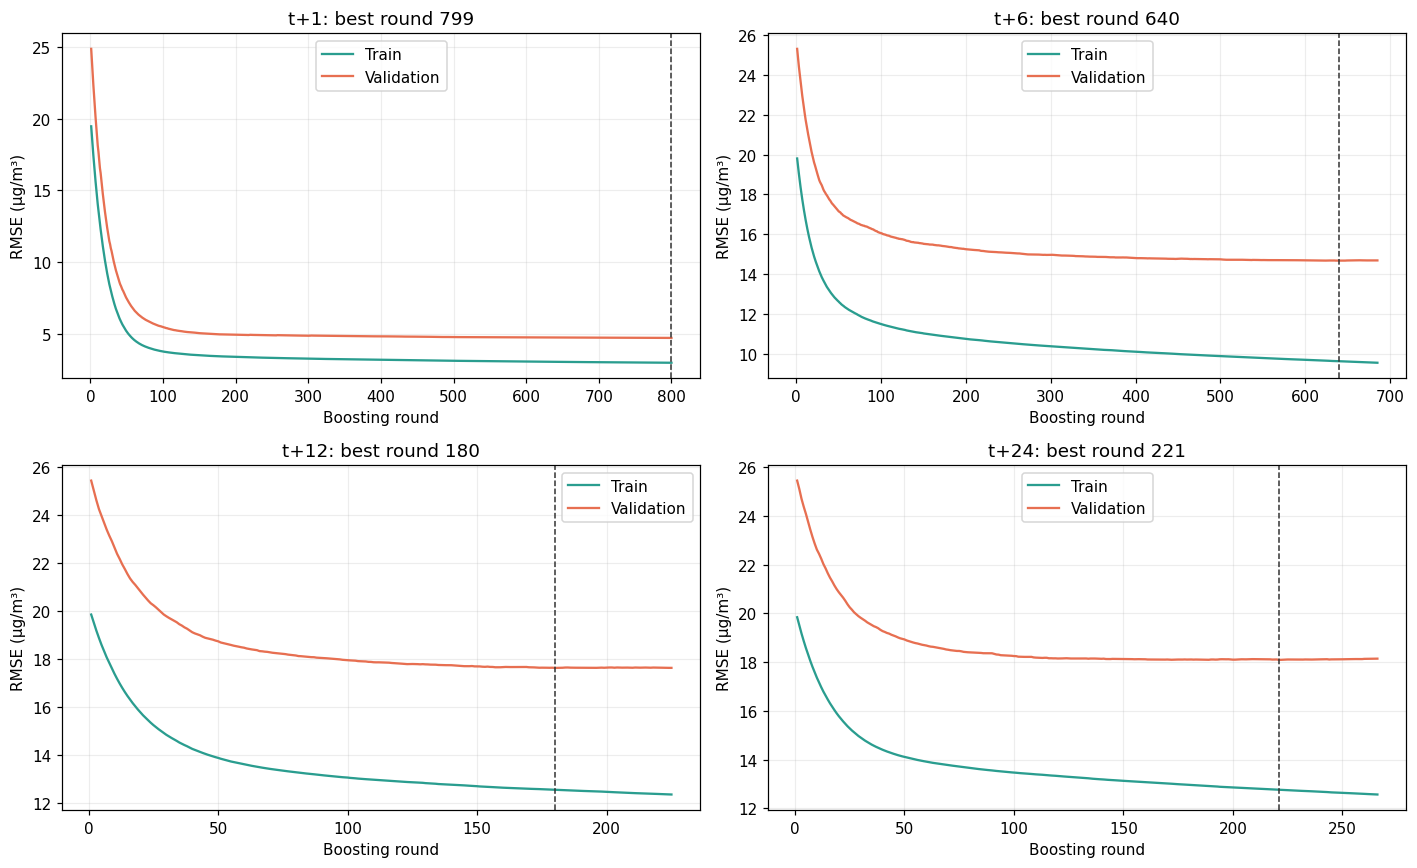
\includegraphics[width=\linewidth,height=0.70\textheight,keepaspectratio]{figures/best_model_learning_curves.png}
\end{column}
\begin{column}{0.22\textwidth}
\footnotesize
\begin{alertblock}{Dấu hiệu}
Khoảng cách Train--Validation tại best round trung bình 4,30 $\mu$g/m$^3$.
\end{alertblock}
\begin{exampleblock}{Biện pháp}
Early stopping chọn vòng tốt nhất và hạn chế overfitting ở horizon dài.
\end{exampleblock}
\end{column}
\end{columns}
\end{frame}

\begin{frame}{4. Kết quả và thảo luận}{Độ quan trọng đặc trưng}
\begin{columns}[T]
\begin{column}{0.60\textwidth}
\includegraphics[width=\linewidth]{figures/best_model_feature_importance.png}\end{column}
\begin{column}{0.37\textwidth}
\begin{itemize}
\item PM2.5 hiện tại.
\item Rolling 12h và 24h.
\item City Hà Nội.
\item Lag ngắn và PM10.
\end{itemize}
\begin{alertblock}{Không phải nhân quả}
Importance chỉ phản ánh mức model sử dụng feature.
\end{alertblock}
\end{column}
\end{columns}
\end{frame}

\begin{frame}{4. Kết quả và thảo luận}{Khoảng conformal 90\%}
\centering
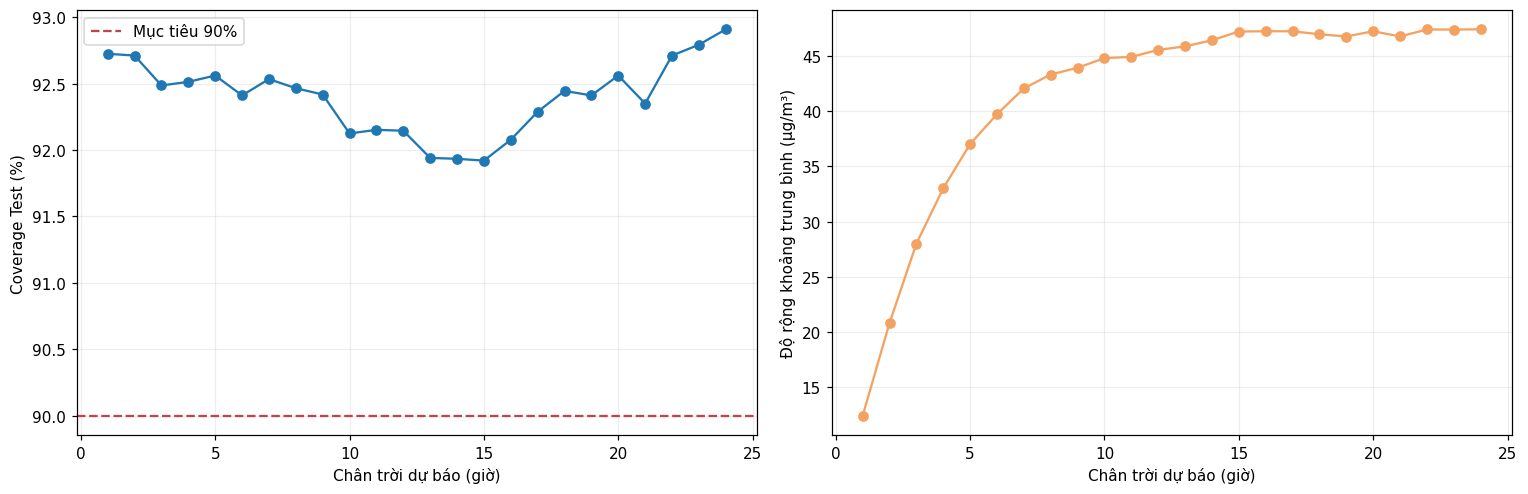
\includegraphics[width=0.88\linewidth]{figures/best_model_conformal_coverage.png}
\small Coverage Test tổng hợp 92,4\%. Hà Nội 89,1\%, TP.HCM 94,9\%, Đà Nẵng 93,2\%; cần hiệu chỉnh lại khi dữ liệu drift.
\end{frame}

\begin{frame}{4. Kết quả và thảo luận}{Dự báo trên phần cuối tập Test}
\centering

\includegraphics[width=0.98\linewidth,height=0.68\textheight,keepaspectratio]{figures/best_model_test_forecast.png}

\footnotesize Lát cắt $t+24$ trên 240 giờ cuối: XGBoost bám xu hướng phổ biến nhưng vẫn làm trơn một số đỉnh, đặc biệt tại Hà Nội; dải xanh là khoảng conformal 90\% hiệu chỉnh từ Validation.
\end{frame}

\begin{frame}{4. Kết quả và thảo luận}{Residual và xu hướng làm trơn đỉnh}
\centering
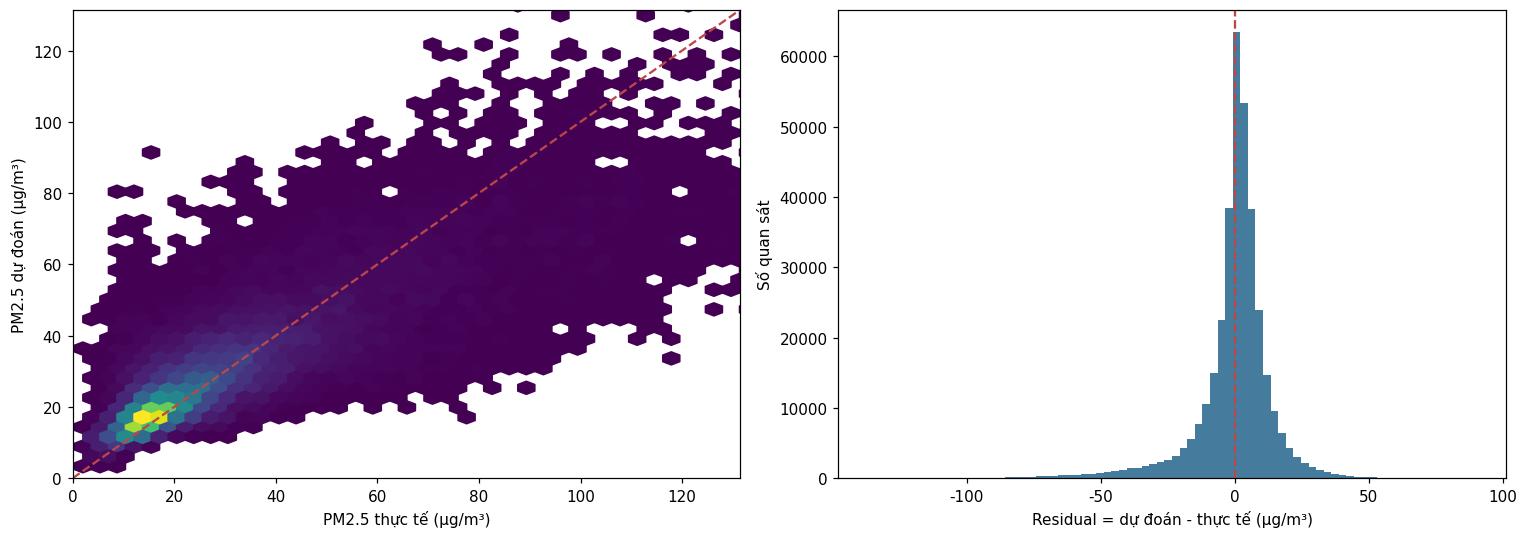
\includegraphics[width=0.94\linewidth]{figures/best_model_residual_analysis.png}
\small Residual tập trung gần 0 ở vùng phổ biến nhưng âm mạnh tại một số đỉnh PM2.5 cao.
\end{frame}

\begin{frame}{4. Kết quả và thảo luận}{Confusion matrix hậu xử lý}
\begin{columns}[T]
\begin{column}{0.59\textwidth}
\includegraphics[height=0.72\textheight]{figures/best_model_confusion_matrix.png}\end{column}
\begin{column}{0.38\textwidth}
\begin{itemize}
\item Macro F1: 0,389.
\item Good recall: 0,130.
\item Very Unhealthy recall: 0,082.
\item Hazardous: không có mẫu Test.
\end{itemize}
\begin{alertblock}{Cách đọc}
Ma trận chỉ chẩn đoán model hồi quy sau khi chia dải do nhóm quy ước.
\end{alertblock}
\end{column}
\end{columns}
\end{frame}

\begin{frame}{4. Kết quả và thảo luận}{Trường hợp sai lớn nhất}
\begin{columns}[T]
\begin{column}{0.54\textwidth}
\begin{block}{Hà Nội, target 25/04/2026 06:00}
\begin{itemize}
\item Horizon: $t+24$.
\item Thực tế: 186,7 $\mu$g/m$^3$.
\item Dự báo: 50,18 $\mu$g/m$^3$.
\item Sai số tuyệt đối: 136,52 $\mu$g/m$^3$.
\end{itemize}
\end{block}
\end{column}
\begin{column}{0.43\textwidth}
\textbf{Giả thuyết nguyên nhân}
\begin{itemize}
\item Đỉnh phát thải đột ngột.
\item CAMS có độ phân giải không gian hạn chế.
\item Mẫu cực đoan hiếm.
\item Squared loss và cây có xu hướng làm trơn.
\end{itemize}
\end{column}
\end{columns}
\end{frame}

\section{5. Ứng dụng web}
\begin{frame}{5. Ứng dụng web}{Kiến trúc triển khai}
\centering
\begin{tikzpicture}[node distance=0.85cm,every node/.style={font=\small}]
\node[draw,rounded corners,fill=blue!8,minimum width=2.5cm,minimum height=0.85cm] (data) {Open-Meteo / CAMS};
\node[draw,rounded corners,fill=green!10,right=of data,minimum width=2.4cm,minimum height=0.85cm] (api) {FastAPI};
\node[draw,rounded corners,fill=orange!12,right=of api,minimum width=2.7cm,minimum height=0.85cm] (model) {24 XGBoost models};
\node[draw,rounded corners,fill=purple!10,right=of model,minimum width=2.4cm,minimum height=0.85cm] (ui) {React / Vite};
\draw[-{Latex}] (data)--(api);\draw[-{Latex}] (api)--(model);\draw[-{Latex}] (model)--(ui);
\node[draw,rounded corners,fill=gray!10,below=of api,minimum width=2.8cm] (history) {Profile lịch sử và cache};
\draw[-{Latex}] (history)--(api);
\end{tikzpicture}
\vspace{0.45cm}
\begin{itemize}
\item Chọn thành phố và horizon 1--24 giờ.
\item Dự báo tự động hoặc nhập kịch bản.
\item Lag và rolling lấy tự động từ lịch sử, không bắt người dùng nhập.
\end{itemize}
\end{frame}

\begin{frame}{5. Ứng dụng web}{Tổng quan và dự báo đa chân trời}
\begin{columns}[T]
\begin{column}{0.49\textwidth}\centering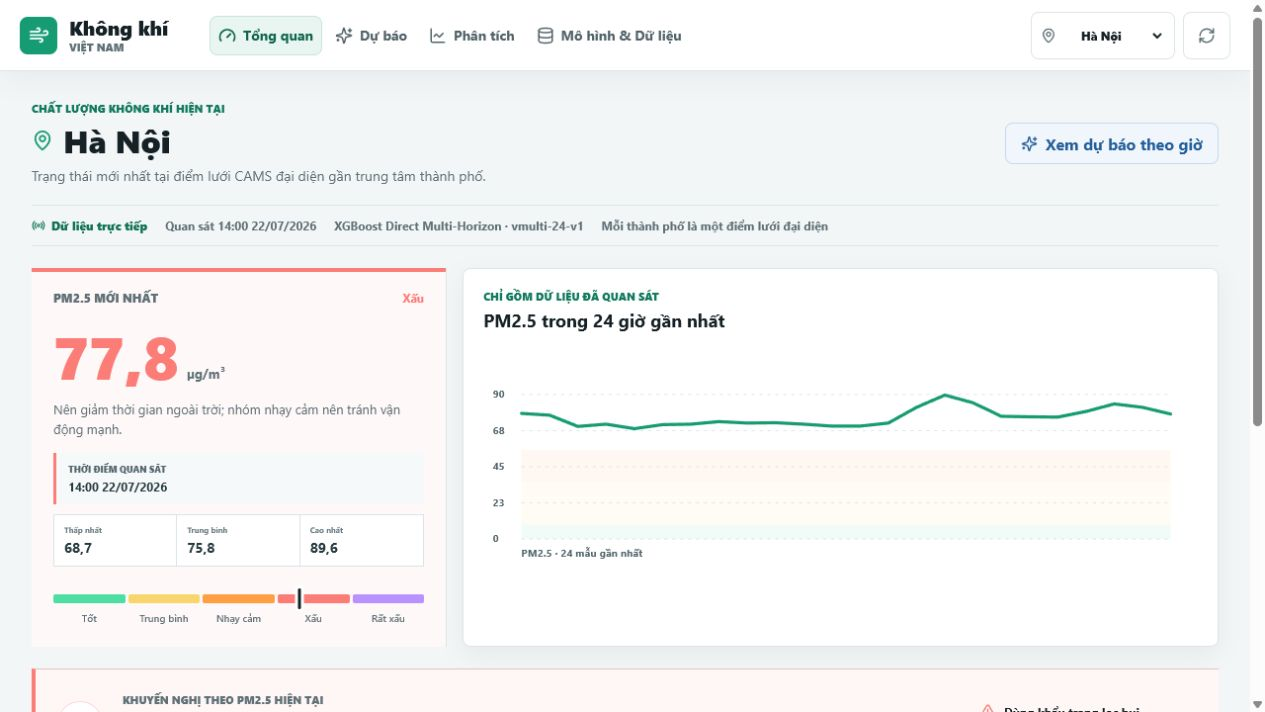
\includegraphics[width=\linewidth]{figures/web_overview.png}\par\scriptsize Tổng quan hiện trạng\end{column}
\begin{column}{0.49\textwidth}\centering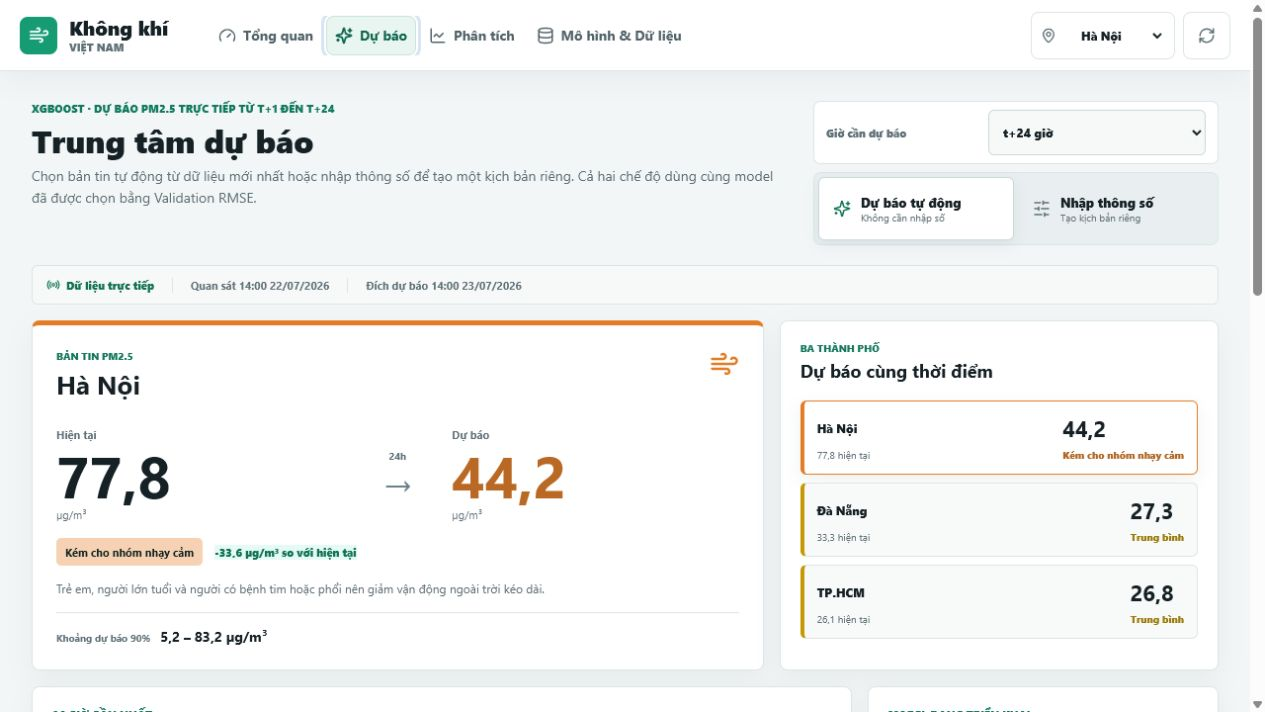
\includegraphics[width=\linewidth]{figures/web_forecast.png}\par\scriptsize Chọn horizon và xem bản tin\end{column}
\end{columns}
\end{frame}

\begin{frame}{5. Ứng dụng web}{Kịch bản nhập tay và phân tích}
\begin{columns}[T]
\begin{column}{0.49\textwidth}\centering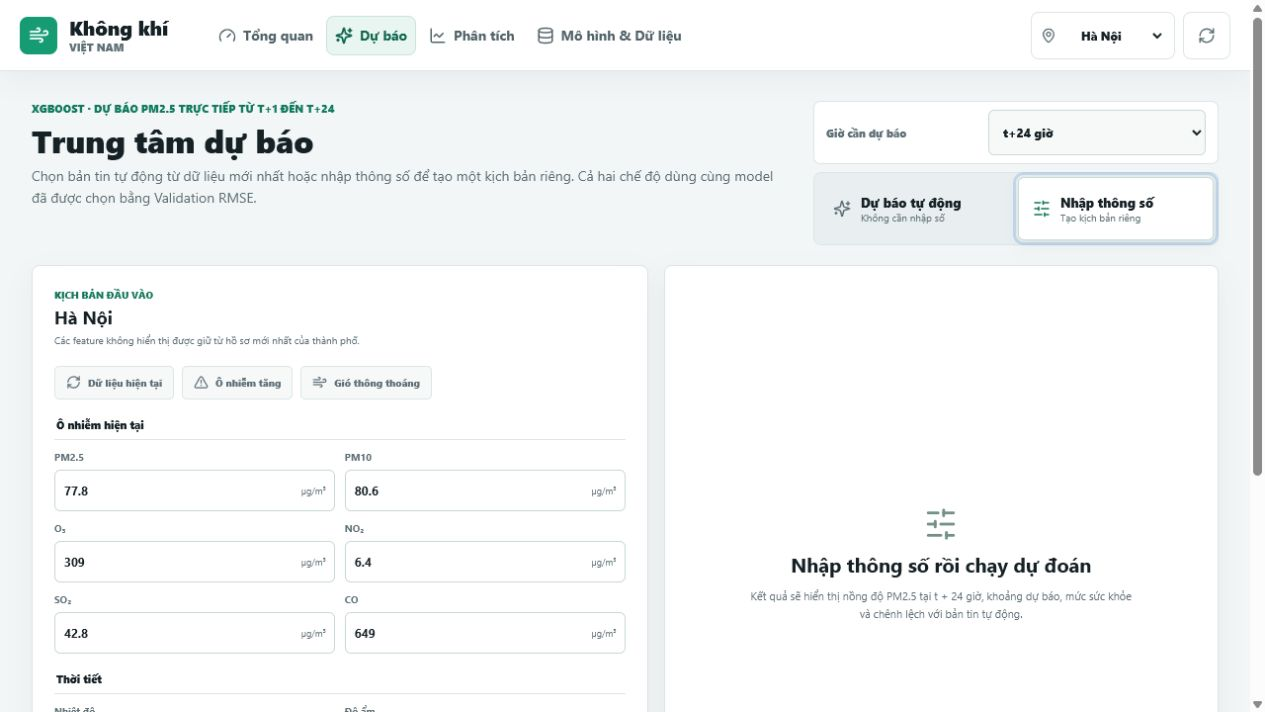
\includegraphics[width=\linewidth]{figures/web_manual_forecast.png}\par\scriptsize Kịch bản người dùng\end{column}
\begin{column}{0.49\textwidth}\centering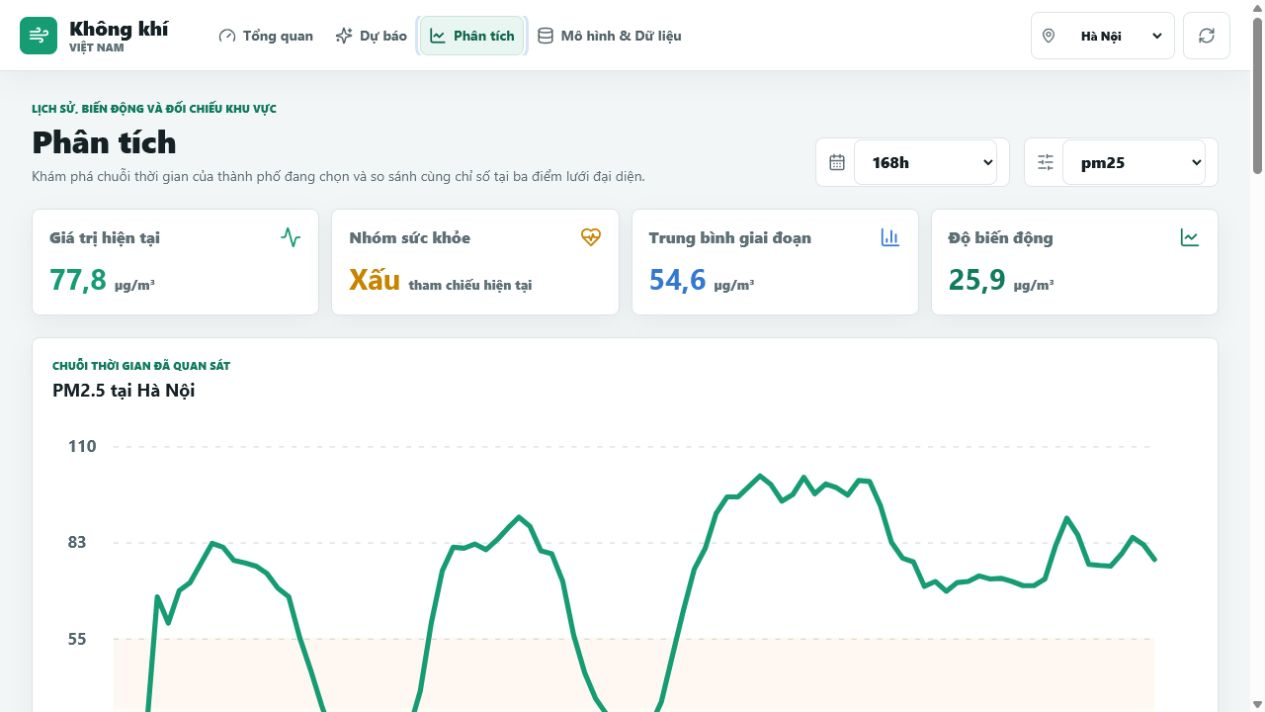
\includegraphics[width=\linewidth]{figures/web_analysis.png}\par\scriptsize Phân tích xu hướng\end{column}
\end{columns}
\end{frame}

\begin{frame}{5. Ứng dụng web}{Minh bạch model và dữ liệu}
\begin{columns}[T]
\begin{column}{0.66\textwidth}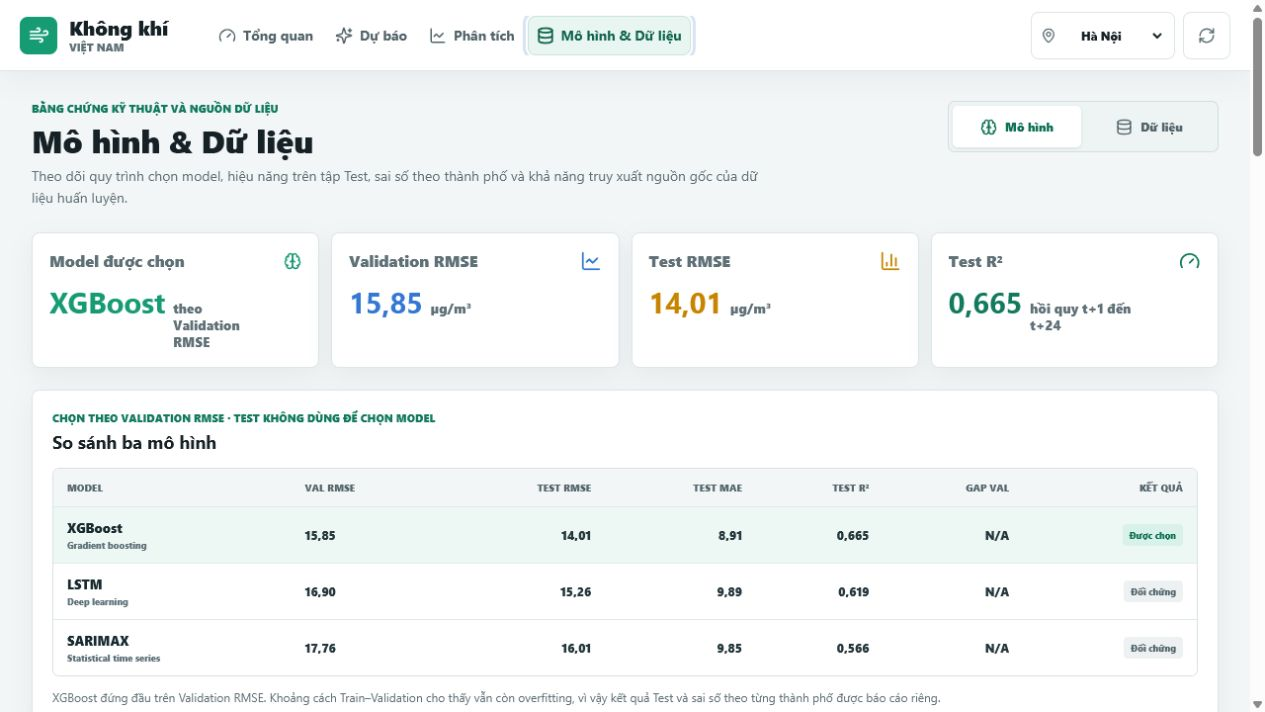
\includegraphics[width=\linewidth]{figures/web_model_data.png}\end{column}
\begin{column}{0.31\textwidth}
\begin{itemize}
\item Công khai model được chọn.
\item Hiển thị metric và learning curve.
\item Nêu nguồn CAMS và giới hạn điểm lưới.
\item API local đã kiểm thử; Docker sẵn cho Render.
\end{itemize}
\end{column}
\end{columns}
\end{frame}

\section{6. Kết luận}
\begin{frame}{6. Kết luận}{Kết quả, hạn chế và hướng phát triển}
\begin{columns}[T]
\begin{column}{0.49\textwidth}
\begin{exampleblock}{Kết quả}
\begin{itemize}
\item Dự báo PM2.5 từ $t+1$ đến $t+24$.
\item XGBoost thắng 5/5 Validation folds.
\item Test RMSE 14,01; MAE 8,91; R$^2$ 0,665.
\item Web cho chọn giờ và hai chế độ dự báo.
\end{itemize}
\end{exampleblock}
\end{column}
\begin{column}{0.49\textwidth}
\begin{alertblock}{Hạn chế và hướng phát triển}
\begin{itemize}
\item CAMS không phải trạm mặt đất.
\item Yếu tại đỉnh hiếm và Hà Nội.
\item Cần strict refit CV, weighted/quantile loss.
\item Giám sát drift, tái hiệu chỉnh conformal.
\item Cần xác minh URL cloud công khai trước khi nộp.
\end{itemize}
\end{alertblock}
\end{column}
\end{columns}
\end{frame}

\begin{frame}
\centering
\Huge\textbf{Cảm ơn thầy/cô và các bạn đã lắng nghe!}\\[0.7cm]
\Large Nhóm 11 - Dự báo PM2.5 đa chân trời
\end{frame}

\end{document}
